\chapter{Discussion}
\label{ch:discu}
This chapter reflects on the results presented in Chapter 4 and discusses how they address
the research questions, the implications of the findings, and possible directions for future
work.
\section{Interpretation of Results}
\subsection{Accuracy and Robustness  }
The results demonstrate that integrating a prior 3D map into a LiDAR-inertial localization framework significantly enhances both accuracy and robustness.By aligning real-time LiDAR scans with globally consistent reference  map , the system reduces drift that typically accumulates in odometry-only methods.Experimental results from multiple datasets show that the proposed system achieves centimeter- to decimeter-level translational RMSE(see  Table ~\ref{tab:ape_rot_saxion_seq1}, \ref{tab:ape_rot_saxion_seq2},  \ref{tab:ape_rot_saxion_seq3}), while standalone LiDAR-Inertial Odometry exhibits drift ranging from meter-level to over ten meters in extended trajectories.Unlike SLAM approaches that rely on loop closures, this method consistently aligns live LiDAR scans to a static reference map, maintaining accuracy even in environments with sparse or unreliable loop opportunities(Table ~\ref{tab:ape_rot_kitti_seq5}).

To effectively combine high-frequency LiDAR-Inertial Odometry (FAST-LIO2) with
NDT-based map matching, the proposed system employs a factor graph optimization frame-
work.The factor graph fuses odometry and scan-matching constraints into a consistent probabilistic model, reducing accumulated linearization errors compared to filtering methods.The sliding-window strategy further ensures real-time performance by limiting the optimization to a fixed temporal window, maintaining constant computational cost regardless of trajectory length (see Figure \ref{fig:sliding_vs_batch}).This
design effectively mitigates drift in odometry and compensates for scan-matching failures,
preserving both short-term precision and long-term consistency in challenging environments.

\subsection{Real-Time Performance }

Results show that while standard NDT and ICP struggle to meet real-time constraints as map size  increases often resulting in slow convergence or failure, the proposed approach maintains reliable performance (Table \ref{tab:scanmap_radius}). By operating on locally segmented submaps and leveraging multithreaded NDT-OMP, the system ensures fast and stable scan matching.To manage computational load in large-scale environments, the system incorporates dynamic submap loading and tile-based map management. Instead of operating on a full global map, only local map tiles within a defined radius are loaded and used for scan-to-map matching. This reduces memory usage and significantly improves convergence speed of multithreaded NDT-OMP matching.The proposed pipeline operates at an average rate of 48 Hz (23 ms per frame), as illustrated in Figure~\ref{fig:computation_summary1}.

\subsection{Environmental Adaptability }
Under moderate fog (visibility {60}{m}), both NDT and the fusion method exhibit stable performance, with {APE} increasing only marginally compared to the baseline(Table ~\ref{tab:ape_fog_translation}). This confirms that {NDT} scan matching retains resilience in moderately degraded visibility. However, under severe fog ({visibility 30}{m}), scan matching becomes unreliable due to poor feature correspondences, and {FAST-LIO2} suffers from high drift. As a result, the fusion pipeline repeatedly fails, unable to maintain reliable pose estimates. 

In sparse map regions and transition zones, scan-to-map registration frequently fails due to a lack of correspondences. Nevertheless, the fusion method maintains localization thanks to high-rate odometry updates and prior structure in the factor graph(Figure~\ref{fig:ape-error-unmapped}).

Dynamic object removal further enhances registration performance. Filtering out transient objects improves convergence, reduces iteration counts, and lowers overall computational load during scan matching(see Table~\ref{tab:dynamic_object_runtime_pipeline_comparison}). While the object detection module introduces some processing overhead, it remains feasible for real-time operation, particularly on GPU-accelerated platforms. However, the system may face limitations on resource-constrained devices without hardware acceleration.

\section{Implications}
These findings underscore the value of combining prior maps, real-time odometry, and probabilistic optimization for autonomous navigation. The approach enables accurate and robust pose estimation in GNSS-denied and moderately degraded visual environments, which are common in urban outdoor and indoor settings. The use of dynamic submap loading and multithreaded NDT further supports the system’s deployment in real-time and large-scale environments, particularly for high-accuracy, repetitive navigation tasks.


\subsection{Limitations and Future Work}

While the proposed localization system demonstrates high accuracy and robustness across diverse scenarios, several limitations remain. First, it assumes a known initial pose, which restricts its ability to perform global localization or recover from kidnapped robot scenarios. Second, the system relies on a static prior map without support for online map adaptation, which limits its effectiveness in long-term or evolving environments.

A further A limitation arises in highly degenerate environments—such as corridors, open plains, or fog—where LiDAR lacks sufficient geometric richness. While FAST-LIO2 and multithreaded NDT are resilient under moderate degradation, their performance degrades in cases of extreme sparsity or planar dominance. FAST-LIO2 relies on consistent local structure for correction, and even NDT-OMP may fail to converge under heavy noise.

To address this, a future enhancement proposes replacing the tightly coupled LIO front-end with a modular graph-based framework, treating IMU data as a pre-integration factor. This would enable pose propagation during LiDAR degradation and support selective correction when reliable map constraints are available. The flexible structure also allows integration of visual or radar factors for improved localization in perceptually degraded scenes. The current and proposed formulations are shown in Figure~\ref{fig:sensor_formulation}, panels (a) and (b), respectively.
In summary, future work may proceed along the following directions:
\begin{itemize}
	\item \textbf{Global localization and recovery:} Integration of coarse initial pose estimation methods for startup or failure recovery.
	\item \textbf{Adaptive mapping:} Support for online map updates or hybrid SLAM fusion during long-term deployments.
	\item \textbf{Modular multi-sensor fusion:} A graph-based architecture incorporating visual, radar, and inertial factors to enhance robustness across sensor failures and environmental degradation.
\end{itemize}

These enhancements would strengthen the system’s applicability in real-world autonomous navigation, particularly in complex, dynamic, and partially observable environments.

\begin{figure}[H]
	\centering
	\begin{subfigure}[t]{0.7\textwidth}
		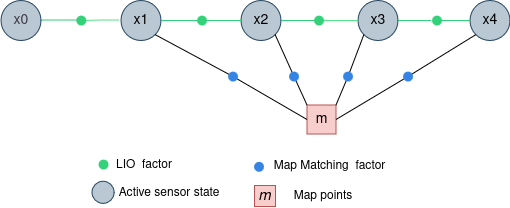
\includegraphics[width=\linewidth]{images/current_factor.drawio.png}
		\caption{Current formulation: tightly coupled LiDAR-Inertial Odometry (FAST-LIO2) with direct map matching via NDT-OMP.}
		\label{fig:current_sensor_fusion}
	\end{subfigure}
	\hfill
	\begin{subfigure}[t]{0.7\textwidth}
		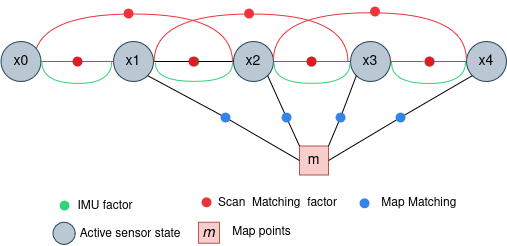
\includegraphics[width=\linewidth]{images/proposed.drawio.png}
		\caption{Proposed formulation: modular factor graph where IMU is treated as a pre-integration factor, allowing flexible integration of additional sensors.}
		\label{fig:proposed_sensor_fusion}
	\end{subfigure}
	
	\caption{Comparison of sensor fusion architectures. (a) The current design integrates FAST-LIO2 with NDT-based map matching in a tightly coupled manner. (b) The proposed approach restructures the system into a modular factor graph, supporting IMU pre-integration and extensibility to visual or radar factors for increased robustness in degraded environments.}
	\label{fig:sensor_formulation}
\end{figure}

